\documentclass[sigconf]{acmart}

\usepackage{algorithmic}
\usepackage{algorithm}
\usepackage{hyperref}
\usepackage[newfloat,cache=false]{minted}

\begin{document}

\title{Lab 3 Exercise - Optimise it!}
\author{Luke McClure}
\email{29573904}

\maketitle
\pagestyle{myheadings}
\section{Exercise 1}
\subsection{Rastrigin}
\begin{listing}[H]
    \begin{minted}[frame=lines, breaklines, breaksymbolleft=, fontsize=\footnotesize]{python}
def rastrigin(x, A=1):
    sx = 0
    for xi in x:
        sx += xi**2 - A*torch.cos(2*np.pi*xi)
    return A*x.shape[0] + sx
\end{minted}
\end{listing}
For the rastrigin function, these optimisers found the following minimums after 100 epochs and with learning rate 0.01.

\begin{center}
    \begin{tabular}{| c c |}
        \hline
        Optimiser & Final Point (100 Epochs) \\ 
        \hline\hline
        SGD & [2.8224, 2.8224] \\
        SGD + Momentum & [-0.9470, -0.9470]\\
        Adagrad & [4.8423, 4.8423]\\
        Adam & [3.9386, 3.9386]\\
        \hline      
    \end{tabular}
\end{center}

SGD with Momentum is the best performing optimiser, falling close to the global minimum but getting stuck in a local minimum. 
Standard SGD falls short at [2.8, 2.8] and has stopped descending further, finding a local minimum to rest in.
\begin{figure}[H]
    \centering
    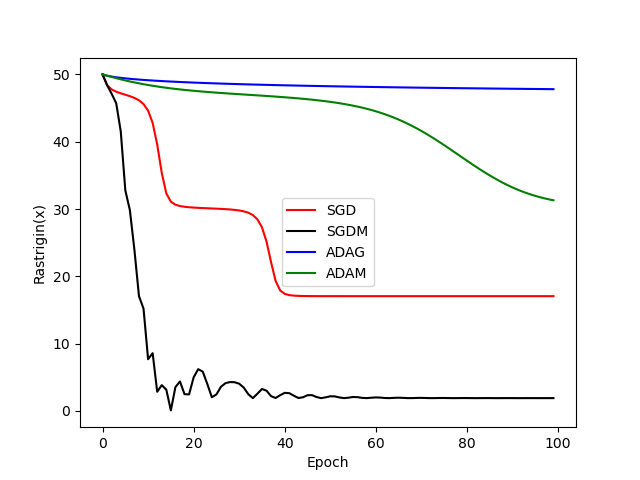
\includegraphics[scale=0.5]{"../optimisers.png"}
\end{figure}
From plotting the loss it is clear that both Adam and Adagrad are still in the process of finding a minimum to rest in after 100 epochs. 
Adam has moved steadily down and is starting to slow but Adagrad has barely moved from the starting position of [5,5] and has a very shallow gradient.

\section{Exercise 2}
\subsection{Iris SVM}
The following code was used to implement a soft-margin SVM. Using this hinge loss will tune the weights to create a boundary separating two classes.
\begin{listing}[H]
    \begin{minted}[frame=lines, breaklines, breaksymbolleft=, fontsize=\footnotesize]{python}
def hinge_loss(y_pred, y_true):
    return torch.mean(torch.max(torch.zeros(y_pred.shape),1-y_pred*y_true))

def svm(x, w, b):
    h = (w*x).sum(1) + b
    return h
    \end{minted}
\end{listing}
The performance of this learning machine was then evaluated using two optimisers.

\begin{center}
    \begin{tabular}{| c c c c |}
        \hline
        Optimiser & Validation Accuracy & Validation Loss & Mean Loss \\ 
        \hline\hline
        SGD & 0.88 & 0.3299 & 0.2100 \\
        Adam & 0.92 & 0.1711 & 0.1843 \\
        \hline      
    \end{tabular}
\end{center}

The initial validation loss from the first run indicates that Adam is a better optimiser for linear-SVMs than SGD. This is confirmed by running 200 iterations with randomly initialised weights and finding a mean loss for both optimisers.

\begin{figure}[H]
    \centering
    \includegraphics[scale=0.5]{"svm.png"}
\end{figure}

Plotting the cumulative mean over 200 runs of both optimisers shows how stable the optimser is to starting conditions.
The fluctuations of the cumulative mean up and down by suggests that an optimiser is not stable and is very dependant on the starting conditions.
It can be seen clearly that SGD both ends at a larger mean value as well as having a much rougher line over the course of all the samples. 
While the Adam optimiser has some large spikes at the start, this is when the sample size is small. The continuing flat trend of the Adam optimizer indicates it is more stable and at a lower loss than SGD.

\end{document}
\endinput